% Radio horizon on the airless Moon, d = sqrt(2 h R_M), for masts, towers and mountains.
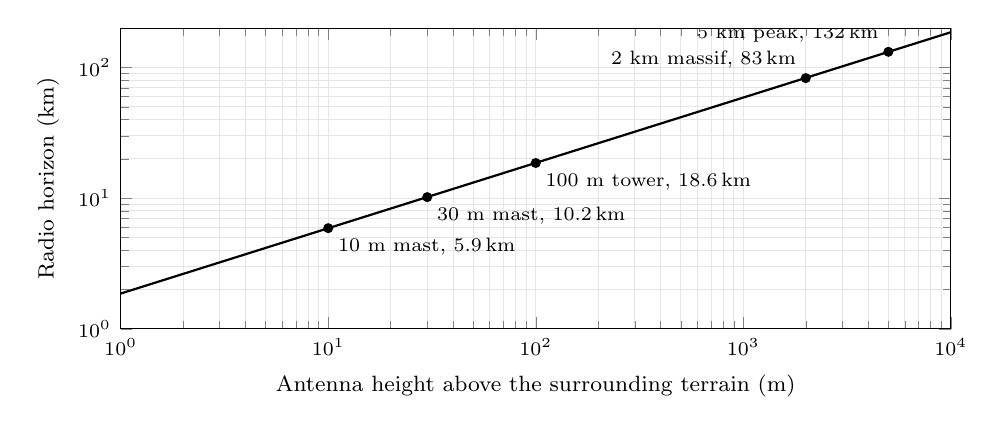
\begin{tikzpicture}
\begin{axis}[
  width=\columnwidth, height=5.4cm, xmode=log, ymode=log,
  xmin=1, xmax=10000, ymin=1, ymax=200,
  xlabel={Antenna height above the surrounding terrain (m)}, ylabel={Radio horizon (km)},
  grid=both, grid style={gray!20}, tick label style={font=\scriptsize}, label style={font=\footnotesize},
]
\addplot[black, thick, domain=1:10000, samples=60] {sqrt(2*x*1737.4e3)/1000};
\addplot[only marks, mark=*, mark size=1.6pt, black] coordinates {(10,5.9)};
\node[font=\scriptsize, anchor=north west] at (axis cs:10,5.9) {10 m mast, 5.9\,km};
\addplot[only marks, mark=*, mark size=1.6pt, black] coordinates {(30,10.2)};
\node[font=\scriptsize, anchor=north west] at (axis cs:30,10.2) {30 m mast, 10.2\,km};
\addplot[only marks, mark=*, mark size=1.6pt, black] coordinates {(100,18.6)};
\node[font=\scriptsize, anchor=north west] at (axis cs:100,18.6) {100 m tower, 18.6\,km};
\addplot[only marks, mark=*, mark size=1.6pt, black] coordinates {(2000,83)};
\node[font=\scriptsize, anchor=south east] at (axis cs:2000,83) {2 km massif, 83\,km};
\addplot[only marks, mark=*, mark size=1.6pt, black] coordinates {(5000,132)};
\node[font=\scriptsize, anchor=south east] at (axis cs:5000,132) {5 km peak, 132\,km};
\end{axis}
\end{tikzpicture}
